\documentclass[tikz,border=6pt]{standalone}
\usepackage{amsmath,amssymb}
\usepackage{tikz}
\usetikzlibrary{arrows.meta}
\newcommand{\ket}[1]{\left|#1\right\rangle}

\begin{document}
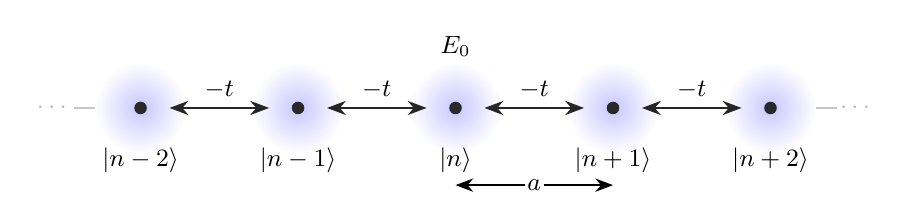
\begin{tikzpicture}[
  >=Stealth,
  site/.style={circle, fill=black!84, inner sep=1.6pt},
  hop/.style={<->, line width=0.85pt, draw=black!85, shorten <=8pt, shorten >=8pt},
  lattice/.style={line width=0.6pt, gray!45},
  every node/.style={font=\small}
]
  \draw[lattice] (-4.85,0) -- (4.85,0);

  \foreach \x in {-4,-2,0,2,4} {
    \shade[inner color=blue!22, outer color=blue!0] (\x,0) circle[radius=0.58];
  }

  \node[site] (s1) at (-4.0,0) {};
  \node[site] (s2) at (-2.0,0) {};
  \node[site] (s3) at (0,0) {};
  \node[site] (s4) at (2.0,0) {};
  \node[site] (s5) at (4.0,0) {};

  \node[below=11pt] at (s1) {$\ket{n-2}$};
  \node[below=11pt] at (s2) {$\ket{n-1}$};
  \node[below=11pt] at (s3) {$\ket{n}$};
  \node[below=11pt] at (s4) {$\ket{n+1}$};
  \node[below=11pt] at (s5) {$\ket{n+2}$};

  \draw[hop] (s1) -- node[above=2pt, fill=white, inner sep=1pt] {$-t$} (s2);
  \draw[hop] (s2) -- node[above=2pt, fill=white, inner sep=1pt] {$-t$} (s3);
  \draw[hop] (s3) -- node[above=2pt, fill=white, inner sep=1pt] {$-t$} (s4);
  \draw[hop] (s4) -- node[above=2pt, fill=white, inner sep=1pt] {$-t$} (s5);

  \draw[<->, line width=0.75pt] (s3) ++(0,-0.98) -- node[fill=white, inner sep=1pt] {$a$} ++(2.0,0);
  \node[above=15pt] at (s3) {$E_0$};
  \node[gray!55] at (-5.1,0) {$\cdots$};
  \node[gray!55] at (5.1,0) {$\cdots$};
\end{tikzpicture}
\end{document}
